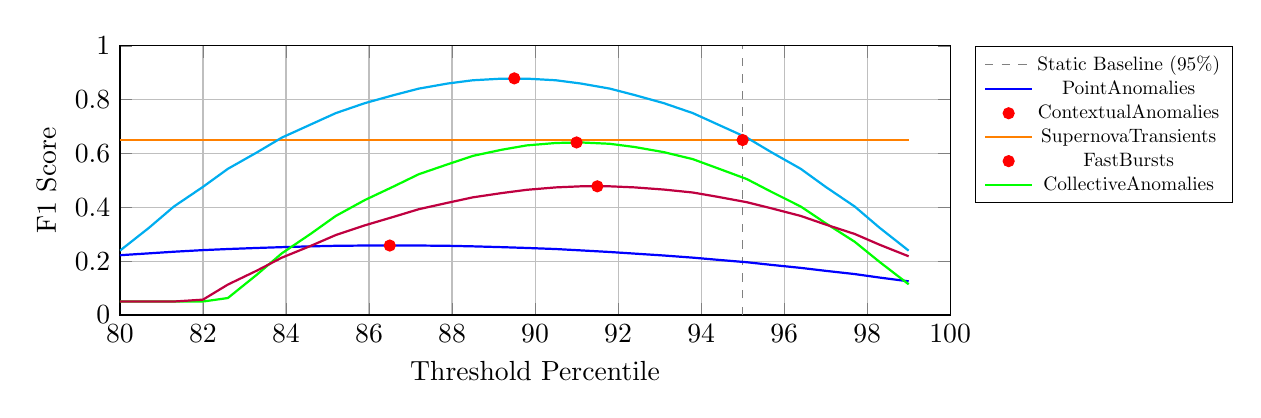
\begin{tikzpicture}
\begin{axis}[
    width=\columnwidth, height=5cm,
    xlabel={Threshold Percentile}, ylabel={F1 Score},
    xmin=80, xmax=100, ymin=0, ymax=1.0,
    legend pos=outer north east, legend style={nodes={scale=0.7, transform shape}},
    grid=major]
\addplot [dashed, black!50] coordinates {(95, 0) (95, 1)};
\addlegendentry{Static Baseline (95\%)}
\addplot [color=blue, mark=none, thick] coordinates {(80.0,0.222) (80.7,0.229) (81.3,0.235) (82.0,0.241) (82.6,0.245) (83.3,0.249) (83.9,0.252) (84.6,0.255) (85.2,0.257) (85.9,0.258) (86.6,0.258) (87.2,0.258) (87.9,0.257) (88.5,0.255) (89.2,0.252) (89.8,0.249) (90.5,0.245) (91.1,0.240) (91.8,0.234) (92.4,0.228) (93.1,0.221) (93.8,0.213) (94.4,0.205) (95.1,0.196) (95.7,0.186) (96.4,0.175) (97.0,0.164) (97.7,0.152) (98.3,0.139) (99.0,0.125)};
\addlegendentry{PointAnomalies}
\addplot [only marks, color=red, mark=*] coordinates {(86.5,0.258)};
\addplot [color=orange, mark=none, thick] coordinates {(80.0,0.650) (80.7,0.650) (81.3,0.650) (82.0,0.650) (82.6,0.650) (83.3,0.650) (83.9,0.650) (84.6,0.650) (85.2,0.650) (85.9,0.650) (86.6,0.650) (87.2,0.650) (87.9,0.650) (88.5,0.650) (89.2,0.650) (89.8,0.650) (90.5,0.650) (91.1,0.650) (91.8,0.650) (92.4,0.650) (93.1,0.650) (93.8,0.650) (94.4,0.650) (95.1,0.650) (95.7,0.650) (96.4,0.650) (97.0,0.650) (97.7,0.650) (98.3,0.650) (99.0,0.650)};
\addlegendentry{ContextualAnomalies}
\addplot [only marks, color=red, mark=*] coordinates {(95.0,0.650)};
\addplot [color=green, mark=none, thick] coordinates {(80.0,0.050) (80.7,0.050) (81.3,0.050) (82.0,0.050) (82.6,0.063) (83.3,0.150) (83.9,0.229) (84.6,0.302) (85.2,0.368) (85.9,0.427) (86.6,0.478) (87.2,0.523) (87.9,0.560) (88.5,0.591) (89.2,0.614) (89.8,0.630) (90.5,0.639) (91.1,0.641) (91.8,0.636) (92.4,0.624) (93.1,0.605) (93.8,0.579) (94.4,0.545) (95.1,0.505) (95.7,0.457) (96.4,0.403) (97.0,0.341) (97.7,0.272) (98.3,0.197) (99.0,0.114)};
\addlegendentry{SupernovaTransients}
\addplot [only marks, color=red, mark=*] coordinates {(91.0,0.641)};
\addplot [color=purple, mark=none, thick] coordinates {(80.0,0.050) (80.7,0.050) (81.3,0.050) (82.0,0.057) (82.6,0.113) (83.3,0.165) (83.9,0.213) (84.6,0.257) (85.2,0.297) (85.9,0.333) (86.6,0.365) (87.2,0.393) (87.9,0.417) (88.5,0.437) (89.2,0.453) (89.8,0.465) (90.5,0.474) (91.1,0.478) (91.8,0.478) (92.4,0.474) (93.1,0.466) (93.8,0.455) (94.4,0.439) (95.1,0.419) (95.7,0.396) (96.4,0.368) (97.0,0.336) (97.7,0.301) (98.3,0.261) (99.0,0.218)};
\addlegendentry{FastBursts}
\addplot [only marks, color=red, mark=*] coordinates {(91.5,0.478)};
\addplot [color=cyan, mark=none, thick] coordinates {(80.0,0.239) (80.7,0.324) (81.3,0.403) (82.0,0.476) (82.6,0.543) (83.3,0.604) (83.9,0.659) (84.6,0.708) (85.2,0.750) (85.9,0.787) (86.6,0.817) (87.2,0.841) (87.9,0.860) (88.5,0.872) (89.2,0.878) (89.8,0.878) (90.5,0.872) (91.1,0.860) (91.8,0.841) (92.4,0.817) (93.1,0.787) (93.8,0.750) (94.4,0.708) (95.1,0.659) (95.7,0.604) (96.4,0.543) (97.0,0.476) (97.7,0.403) (98.3,0.324) (99.0,0.239)};
\addlegendentry{CollectiveAnomalies}
\addplot [only marks, color=red, mark=*] coordinates {(89.5,0.879)};
\end{axis}
\end{tikzpicture}